\chapter{Methods}
\label{ch:methods}

\section{\gls{r} -- statistical programming language}
\label{sec:r}

All statistical analyses and data manipulation were carried out with \gls{r} (version 3.3.2 -- ``Sincere Pumpkin Patch''), a free open-source programming language and software environment for statistical computing and graphics \citep{R2016}.

\section{Cancer data}
\label{sec:data}

The raw microarray data from the \citet{Creighton2012}, \citet{Fuentes-Mattei2014} and \citet{Gatza2010a}  studies were downloaded from the \gls{geo} website (\citealp{Edgar2002}; \citetalias{GEO}).
In addition to these breast cancer data sets, the raw microarray data set from a cohort of \gls{nz} breast cancer patients used in the \citet{Print2016} study was downloaded from the \gls{geo} website (abbreviated as \gls{nzbc} data hereafter).
\gls{rnaseq} and clinical data of multiple different cancer types were downloaded from the \gls{icgc} (\citetalias{ICGC}; \citealp{Zhang2011}) and \gls{tcga} \citepalias{TCGA} websites, respectively.

\subsection{Breast cancer data}
\label{sub:breast_cancer_data}

\subsubsection{\citet{Creighton2012} data}
\label{ssub:creighton2012_data}

The raw Affymetrix HGU\-133A microarray gene expression data files from the \citet{Creighton2012} study were downloaded from the \gls{geo} database (\gls{geo} accession ID: GSE24185).
Clinical data of the samples (age, ethnicity, tumour grade, menopause status, \gls{bmi}, \gls{er} status, \gls{pr} status, \gls{her2} status, and \gls{ln} status) were obtained from the Supplementary Table 1 from the \citet{Creighton2012} study.
799 obesity associated gene probes identified in the \citet{Creighton2012} study were obtained from the Supplementary Data File 1 from the \citet{Creighton2012} study.

\subsubsection{\citet{Fuentes-Mattei2014} data}
\label{ssub:fuentes-mattei2014_data}

The raw Affymetrix HGU\-133A microarray gene expression data files from the  \citet{Fuentes-Mattei2014} study were downloaded from the \gls{geo} database (\gls{geo} accession ID: GSE\-20194).
Clinical data for the samples (age, ethnicity, tumour grade, \gls{er}/\gls{pr}/\gls{her2} statuses, and treatments used) in this study was also downloaded from the \gls{geo} database (same \gls{geo} accession ID).
Patient height, weight and \gls{bmi} information were not available in this data set.
130 obesity associated gene probes identified by \citet{Fuentes-Mattei2014} were taken from the Supplementary Table 3 from their paper.

\subsubsection{\acrfull{nzbc} data}
\label{ssub:nzbc_data}

To provide an insight into the relevance of the obesity associated genetic signatures in \gls{nz} patient cohort, the \gls{nzbc} data set used by \citet{Print2016} were used.
The raw Affymetrix HGU133A microarray gene expression data files from the \citet{Print2016} study were downloaded from the \gls{geo} database (\gls{geo} accession ID: GSE3\-6771).
Clinical data for the samples (age, ethnicity, tumour grade, breast cancer subtype, \gls{er}/\gls{pr} statuses, \gls{ln} status, \gls{bmi} and treatments used) in this study was obtained from Prof. Cris Print (personal communication with Assoc. Prof. Mik Black).

\subsubsection{\citet{Gatza2010a} data}
\label{ssub:gatza2010a_data}

The raw microarray gene expression data files from the \citet{Gatza2010a} study were downloaded from the \gls{geo} database (\gls{geo} accession ID: GSE1456, GSE\-1561, GSE2034, GSE3494, GSE4922 and GSE6596).
Only the Affymetrix HGU\-133A microarray samples were included in this project, as the other microarray data from the \citet{Creighton2012}, \citet{Fuentes-Mattei2014} and \citet{Print2016} studies were analysed using the Affymetrix HGU-133A platform.
Clinical data for the samples in \citet{Gatza2010a} study was not available, as these samples were a combination of many different datasets.
The Akt, \gls{bcat}, E2F1, \gls{egfr}, \gls{er}, \gls{her2}, \gls{ifna}, \gls{ifny}, Myc, p53, p63, \gls{pi3k}, \gls{pr}, Ras, \gls{stat3}, Src, \gls{tgfb}, and \gls{tnfa} pathway associated genetic signatures were used by Gatza \textit{et al.}, and the gene probes of all the pathway associated genetic signatures were obtained from the Supplemental Table 10 from their paper.

\subsubsection{Gene probe ID conversion}
\label{ssub:gene_probe_id_conversion}

All of the microarray data used gene probe IDs to refer to the genes, and therefore these probe IDs had to be converted into their corresponding gene symbols.
The gene probe IDs in the raw data were converted into their corresponding gene symbols using the \textit{hgu133a.db} package in \gls{r} \citep{hgu133}.
Since multiple gene probe sets match back to a single gene of interest in a microarray chip, there were conflicting expression data for some of the genes after the conversion of the gene probe sets into gene symbols.
For the gene symbols that had multiple probe set entries, a single probe set was chosen to represent the gene symbol by using the \texttt{collapseRows} function in the \textit{WGCNA} package in \gls{r}, using the default parameters (which chose the probe set with a maximum mean expression value) \citep{Langfelder2008}.
Likewise, any obesity associated or pathway associated gene probes were converted into gene symbols.

\begin{table}[htpb]
	\centering
	\caption{Number of samples in each of the breast cancer microarray data}
	\label{tab:num_sample_microarray}
	\begin{tabular}{lc}
		Data set & Number of samples\\
		\hline
		\hline
		\rule{0pt}{2.25ex}Creighton \textit{et al.} & 103\\
		Fuentes-Mattei \textit{et al.}              & 278\\
		\gls{nzbc}                                  & 99 \\
		Gatza \textit{et al.}                       & 1060\\
		\hline
		\hline
	\end{tabular}
\end{table}

\begin{ThreePartTable}
		\centering
	\begin{TableNotes}
		\begin{footnotesize}
			\item [1] Not available.
		\end{footnotesize}
	\end{TableNotes}
	
	\newpage
	\begin{longtable}{lccc}
		\caption{Summary of the clinical variables in the Creighton \textit{et al.},  Fuentes-Mattei \textit{et al.} and \gls{nzbc} microarray data}
		\label{tab:clin_summary}\\
		Clinical variable & Creighton \textit{et al.} & Fuentes-Mattei \textit{et al.} & \gls{nzbc} \\
		\hline
		\hline
		\endfirsthead
		\multicolumn{3}{c}{\tablename\ \thetable{}\ (continued)}\\
		\hline
		\hline
		\endhead
		\rule{0pt}{2.25ex}Age \\
		\hspace{1em} Min.                    & 30 & 26 & 31 \\
		\hspace{1em} Max.                    & 72 & 79 & 92 \\
		\hspace{1em} Mean                    & 49 & 52 & 59 \\
		\hspace{1em} Median                  & 48 & 51 & 60 \\
		\hline
		\rule{0pt}{2.25ex}Ethnicity         \\
		\hspace{1em} Caucasian        & 77 & 176 & 71 \\
		\hspace{1em} African-American & 16 & 29  & 0  \\
		\hspace{1em} \gls{nz} M\=aori & 0  & 0   & 10 \\
		\hspace{1em} Pacific Islands  & 0  & 0   & 14 \\
		\hspace{1em} Asian            & 10 & 18  & 4  \\
		\hspace{1em} Other            & 0  & 55  & 0  \\
		\hline
		\rule{0pt}{2.25ex}\gls{bmi} status  \\
		\hspace{1em} Normal weight           & 36 & NA\tnote{1} & 28 \\
		\hspace{1em} Overweight              & 29 & NA & 28 \\
		\hspace{1em} Obese                   & 38 & NA & 43 \\
		\hline
		\rule{0pt}{2.25ex}Menopause status  \\
		\hspace{1em} Premenopause            & 49 & NA & NA\\
		\hspace{1em} Perimenopause           & 9  & NA & NA \\
		\hspace{1em} Postmenopause           & 45 & NA & NA \\
		\hline
		\rule{0pt}{2.25ex}Tumour grade      \\
		\hspace{1em} 1                       & 14 & 13 & 11 \\
		\hspace{1em} 2                       & 35 & 104 & 39 \\
		\hspace{1em} 3                       & 54 & 150 & 49 \\
		\hline
		\rule{0pt}{2.25ex}\gls{er} status   \\
		\hspace{1em} \gls{er}$^+$            & 58 & 164 & 72 \\
		\hspace{1em} \gls{er}$^-$            & 42 & 114 & 27 \\
		\hspace{1em} Unknown                 & 3  & 0  & 0  \\
		\hline
		\rule{0pt}{2.25ex}\gls{pr} status   \\
		\hspace{1em} \gls{pr}$^+$            & 48 & 121 & 62 \\
		\hspace{1em} \gls{pr}$^-$            & 50 & 157 & 37 \\
		\hspace{1em} Unknown                 & 5  & 0  & 0  \\
		\hline
		\rule{0pt}{2.25ex}\gls{her2} status \\
		\hspace{1em} \gls{her2}$^+$          & 12 & 59 & NA \\
		\hspace{1em} \gls{her2}$^-$          & 54 & 219 & NA \\
		\hspace{1em} Unknown                 & 37 & 0 & NA \\
		\hline
		\rule{0pt}{2.25ex}\gls{ln} status   \\
		\hspace{1em} \gls{ln}$^+$            & 14 & NA & 56\\
		\hspace{1em} \gls{ln}$^-$            & 89 & NA & 40\\
		\hspace{1em} Unknown                 & 0  & NA & 3 \\
		\hline
		\hline
		\insertTableNotes
	\end{longtable}
\end{ThreePartTable}

\subsection{\gls{icgc} cancer data}
\label{sub:icgc_cancer_data}

\subsubsection{\gls{rnaseq} and clinical data}
\label{ssub:rnaseq_and_clinical_data}

The clinical data for all available cancer types (33 types in total) were downloaded from \gls{tcga} database (last accessed 1 April 2015) and were checked for both the height and weight data for each sample.
Any cancer type with no height and/or weight data for the samples was excluded from the project, as no \gls{bmi} information can be obtained without these data.
Out of these 33 cancer types with clinical data, 14 cancer types had both height and weight data.
However, only 8 cancer types out of these 14 types had \gls{rnaseq} data available from the \gls{icgc} database (last accessed 7 September 2015), so only those 8 cancer types were downloaded and used in this project.
The selected cancer types were: \gls{blca}, \gls{cesc}, \gls{coad}, \gls{kirp}, \gls{lihc}, \gls{read}, \gls{skcm}, \gls{ucec}.

\subsubsection{Data formatting and processing}
\label{ssub:data_formatting_and_processing}

The raw \gls{rnaseq} data from the \gls{icgc} database were formatted so that the count data of all the genes were listed for one sample, then the count data for all the genes for the next sample, and so on.
This data format was highly inconvenient for later analyses so the data were reformatted into a ``gene by sample'' matrix format using the \textit{dplyr} package in \gls{r}.

Another problem with the data was the sample ID in the \gls{rnaseq} data.
Though similar to the \gls{tcga} sample IDs, the \gls{icgc} IDs in the \gls{rnaseq} data had an extra identification code in the sample names.
To associate each sample in the raw \gls{rnaseq} data from the \gls{icgc} database with the correct samples in the clinical data from the \gls{tcga} database, the \gls{icgc} IDs were re-coded to match the \gls{tcga} IDs.
After the IDs were re-coded, samples were checked to see if there were any duplicates in either the \gls{icgc} \gls{rnaseq} data or the \gls{tcga} clinical data.
Where there was a duplicate in the sample ID, a single sample with the highest mean expression value was chosen to represent that particular ID by using the \texttt{collapseRows} function in the \textit{WGCNA} package in \gls{r} \citep{Langfelder2008}.

Since some of the samples did not have either height or weight data, these samples were removed from the analyses.
In each of the eight cancer types, the \gls{tcga} sample IDs in the clinical data were cross-checked with the sample IDs in the \gls{rnaseq} data, and vice versa.
Any samples that did not have either the patient \gls{bmi} information or the \gls{rnaseq} data were removed from the analyses.
This ensured that both \gls{bmi} and \gls{rnaseq} data were available for all of the samples that were included in this project.
See \cref{tab:samplesize} for a summary of the total number of samples included in the analyses for each cancer type.
Where missing, \cref{eq:bmicalc} was used to calculate the \gls{bmi} of the samples in all of the cancer data with height and weight data available (\cref{sec:data}).
\\

\begin{equation}
	\label{eq:bmicalc}
	\gls{bmi} = \frac{Weight (kg)}{Height^2(m^2)}\\
\end{equation}
\\

\noindent
Samples were classified as normal weight (\gls{bmi} \textless{} 25), overweight (25 $\leq$ \gls{bmi} \textless{} 30) or obese (\gls{bmi} $\geq$ 30) based on the \gls{who} definition (\cref{tab:whobmiclass}).
\cref{eq:bmicalc,tab:whobmiclass} were used to calculate and group the patients from the \gls{icgc} cancer data into appropriate \gls{bmi} classes (\cref{tab:icgc_bmi}).

\begin{table}[p]
	\caption{Summary of the total number of samples included in the analyses for each cancer type}
	\label{tab:samplesize}
	\begin{center}
		\begin{tabular}{lcc}
			Cancer Type   & Initial number of samples & Number of samples after exclusion\\
			\hline
			\hline
			\rule{0pt}{2.25ex}BLCA & 295 & 261   \\
			CESC                   & 259 & 224   \\
			COAD                   & 428 & 226   \\
			KIRP                   & 222 & 124   \\
			LIHC                   & 294 & 264   \\
			READ                   & 154 & 73    \\
			SKCM                   & 430 & 218   \\
			UCEC                   & 508 & 482   \\
			\hline
			\hline
		\end{tabular}
	\end{center}
\end{table}

\begin{table}[p]
	\caption{\gls{who} defined \gls{bmi} classification}
	\label{tab:whobmiclass}
	\begin{center}
		\begin{tabular}{lc}
			Classification & \gls{bmi} Value\\
			\hline
			\rule{0pt}{2.25ex}Underweight & \textless{} 20.0\\
			Normal weight/lean & 20.0$\sim$24.9\\
			Overweight & 25.0$\sim$29.9\\
			Obese & $\geq{}$ 30.0\\
			\hline
			\hline
		\end{tabular}
	\end{center}
\end{table}

\begin{table}[p]
	\caption{Summary of the patient \gls{bmi} status in the \gls{icgc} cancer data}
	\label{tab:icgc_bmi}
	\begin{center}
		\begin{tabular}{lcccc}
			& \multicolumn{4}{c}{Number of samples}\\
			\cmidrule(r){2-5}
			Cancer type & Normal weight & Overweight & Obese & Total\\
			\hline
			\hline
			\rule{0pt}{2.25ex}BLCA & 103 & 97  & 61  & 261 \\
			CESC                   & 83  & 64  & 77  & 224 \\
			COAD                   & 75  & 81  & 70  & 226 \\
			KIRP                   & 26  & 53  & 45  & 124 \\
			LIHC                   & 139 & 76  & 49  & 264 \\
			READ                   & 22  & 36  & 15  & 73  \\
			SKCM                   & 71  & 74  & 73  & 218 \\
			UCEC                   & 88  & 108 & 286 & 482 \\
			\hline
			\hline
		\end{tabular}
	\end{center}
\end{table}

\section{Data processing}
\label{sec:datproc}

\subsection{Data normalisation}
\label{sub:data_normalisation}

Any experimental procedure is prone to errors due to differences in experimental conditions, machinery used to measure signals and technical procedures in different laboratories, just to name a few.
All of the data were normalised to remove such experimental bias, errors and noise, so only the true biological signals are considered in the analyses.

\subsubsection{Microarray data}
\label{ssub:microarray_data}

In Affymetrix HGU133A microarray experiments, there are two types of probes present on the microarray chips: \gls{pm} and \gls{mm} probes \citep{Irizarry2003}.
As the name suggests, \gls{pm} probes represent the probes that should perfectly match the gene of interest, whereas \gls{mm} probes have there 13th base pair intentionally altered to measure non-specific binding of the gene \citep{Irizarry2003}.
Various normalisation methods make use of \gls{pm} and \gls{mm}, or ``probe pairs'', to identify true signals from the noise.

\Gls{mas} and \gls{rma} normalisation methods are both part of the \textit{affy} package in \gls{r} \citep{Gautier2004}.
\Gls{mas} uses a difference-based method where it subtracts a value derived from \gls{mm} from \gls{pm}, but this approach may introduce additional noise and/or errors in some cases \citep{Irizarry2003}.
The \gls{rma} method is based on the observation that \gls{pm} is a mixture of background and true signal, and uses mathematical models to estimate the expression while correcting for background signals from \gls{pm} only \citep{Irizarry2003}.
In fact, the \gls{rma} method showed better identification of the true signals than the other methods, including \Gls{mas} method \citep{Irizarry2003}.

The raw microarray data were normalised using both \gls{rma} and \gls{mas} methods, each done separately on a copy of the data.
The reason why the \gls{mas} method was used as well as the \gls{rma} method was because the \gls{mas} normalisation method was used in the \citet{Gatza2010a} study.
Though the normalisation methods were not specified in the \citet{Creighton2012} and \citet{Fuentes-Mattei2014} studies, to allow for data comparison between different datasets and accurate result validation of some of the studies, both \gls{rma} and \gls{mas} methods were considered for normalising the microarray data.

\subsubsection{RNA-seq data}
\label{ssub:rna_seq_data}

\gls{rnaseq} data are fundamentally different to microarray data, as \gls{rnaseq} data is a count data of transcript fragments, while microarray data is a continuous data based on the intensity of the probe pairs.
This means that \gls{rnaseq} data must be processed in a different manner to microarray data.
However, by analysing \gls{rnaseq} data as a count data, it limits the range of statistical tools and types of analyses that can be done on the data, as many tools are designed for normally distributed data like the light intensity measures from the microarray data \citep{Law2014}.

To overcome this limitation, \citet{Law2014} developed a method called ``variance modelling at the observational level'', or ``voom'', that allows any \gls{rnaseq} data to be used in ``any statistical pipeline for microarray data that is precision weight aware''.
In brief, voom first constructs a standard deviation trend from the logged \gls{cpm} value of the genes (experimental design, treatment conditions and other factors are taken into account).
This trend is then used to interpolate the standard deviation of the observation based on its predicted count size, and the inverse square of the predicted standard deviation is used as the weight  for that observation.
The weights of the observations and the logged \gls{cpm} can then be used in other statistical pipelines that allow the input of quantitative weights \citep{Law2014}.

The raw \gls{rnaseq} data were normalised in two different ways depending on the analysis.
For gene expression analyses (\cref{sec:gene_expression_analysis}) and pathway enrichment analyses (\cref{sec:pathway_enrichment_analysis}), voom normalisation from the \textit{limma} package in \gls{r} was used to normalise the data \citep{Ritchie2015}.
For the purposes of data visualisation (\cref{sec:plot_creation}) or the application of the metagene transformation matrices (\cref{sub:svd}) on the \gls{rnaseq} data, the raw data had 1 added (to prevent logging of 0) and then logged to the base of 10.

\subsection{Data standardisation}
\label{sub:data_standardisation}

For metagene creation and data visualisation that used heatmaps, the data were standardised so that each gene in the data had a \gls{m} of 0 and a \gls{sd} of 1.
Since the expression levels of the genes could vary substantially (some may have very low expression, whereas another may have very high expression), the direct comparison of the raw expression values between different genes was not feasible.
Standardisation of each gene allowed the expression levels to be on the same scale, thus allowing better visualisation with heatmaps and comparison between different genes was made possible.

\subsection{Residual data creation}
\label{sub:residual_data_creation}

In some analyses, the Creighton \textit{et al.} data was adjusted for clinical variables to remove any confounding effects from the variables.
For example, a gene from the raw data might have a strong association with \gls{bmi}, but it is possible that other clinical variables such as \gls{er} status and/or tumour grades are also associated with the gene.
To prevent such confounding effect, all of the clinical variables except those that are of interest were adjusted with the use of linear models.

A linear model was created from the Creighton \textit{et al.} data with age, ethnicity, menopause status, tumour grade, hormone (\gls{er}, \gls{pr}, and \gls{her2}) statuses  and \gls{ln} status included in the model.
In addition to this model, another linear model was constructed with the Creighton \textit{et al.} data with only the Caucasian patients included in the data to completely remove the effect of ethnicity (same clinical variables were controlled for, except ethnicity).
Once a linear model was fitted to the Creighton \textit{et al.} data, the remaining data, or the ``residual data'', represented the data that had been corrected for the effects of the unwanted variables, and was used in the analyses that required focus on certain variables without the other variables affecting the result.

\subsection{Batch correction}
\label{sub:batch_correction}

It is most likely that experiments are done at different time period, location and laboratory environment.
These differences between experiments introduces systematic non-biological differences or ``batch effects'' into the data, making it difficult to directly compare the data from different batches \citep{Johnson2007}.
The problem with the batch effect is that the normalisation methods do not control and adjust for the effect \citep{Johnson2007}.
Fortunately, \citet{Johnson2007} developed a method to correct for batch effects in the data, using an empirical Bayesian framework.

The data used in \citet{Gatza2010a} study was a combination of multiple microarray data from various studies, so the batch effect had to be corrected before any analysis was carried out.
Each microarray dataset was normalised with either \gls{rma} or \Gls{mas} separately then combined together into a single dataset, and the batch effect was corrected with the \texttt{ComBat} function (an implementation of the batch correcting method by \citet{Johnson2007}) from the \textit{sva} package in \gls{r} \citep{Leek2012}.

\gls{icgc} cancer data were also corrected for batch effect for the pathway enrichment analysis (\cref{sec:pathway_enrichment_analysis}).
Two combined data sets were created with the \gls{icgc} data.
The first data set was created by voom normalising each cancer data set separately, combine all of the normalised cancer data sets into one, then applied batch correction to the data set (\cref{sub:batch_correction}).
The second data set was created by first combining the cancer data sets into one, then the combined data was voom normalised, and then the batch effect was corrected to obtain the final data set.

\subsection{Sample randomisation in simulation analysis}
\label{sub:sample_randomisation_in_simulation_analysis}

In some cases, an analysis was repeated a number of times to provide statistical evidence that the observed results did not occur by chance.
All of the simulated results must be derived from a randomised data, and by comparing the observed results with the results that occurred by chance, simulation analysis provides statistical evidence for the observed results.
When a simulation was required, none of the values in the original data were modified, but instead the values in the original data were assigned randomly to different samples; in other words, the samples were shuffled.
This provided a random set of data in which a simulation could be conducted with.
The samples were shuffled with the \texttt{sample} function from the \textit{base} package in \gls{r}, and were reshuffled for each simulation.

\section{Gene expression analysis}
\label{sec:gene_expression_analysis}

For gene expression analysis, or differential expression analysis, the \textit{limma} package in \gls{r} was used \citep{Ritchie2015}.
Since there were thousands of genes to be hypothesis tested, adjustment for multiple hypothesis testing had to be considered in order to identify the truly \glspl{deg}.

\subsection{Limma}
\label{sub:limma}

\textit{limma} is a package that contains variety of tools to analyse gene expression data using linear models-based methods, developed by \citet{Ritchie2015}.
For gene expression analysis, \textit{limma} package fits a linear model in a gene-wise manner and produce test statistics that allow the assessment of whether the gene is differentially expressed or not between certain groups of samples \citep{Ritchie2015}.
In this project, the gene expression analysis was carried out to identify \glspl{deg} in the samples that were obese compared to the samples that were non-obese group.

Before the data was analysed using the \textit{limma} analysis pipeline, it was normalised as described in \cref{sub:data_normalisation}: \nameref{sub:data_normalisation}.
In addition to this, a design matrix that describes the experimental design (obese versus non-obese) was created from the clinical data.
To create the design matrix, the samples were divided into two groups, the obese group and the non-obese group, and the constructed group information was used in the \texttt{model.matrix} function (in \textit{limma} package) to form the design matrix.

The \texttt{lmFit} function (\textit{limma}) was used to fit a linear model to the normalised data, using the experimental design information from the design matrix.
The output of this function was used in the \texttt{eBayes} function (\textit{limma}) to identify the \glspl{deg} from the data.
In the \texttt{eBayes} function, statistical parameters are estimated from the data and these parameters are used in the empirical Bayes approach to calculate the summary statistics used for the ranking and identification of \glspl{deg} \citep{Smyth2004}.

The summary statistics from the \texttt{eBayes} function can be displayed with the \texttt{topTable} function (\textit{limma}) and includes the estimate of the fold change of the gene expression in log$_2$, average gene expression level in log$_2$, moderated \textit{t}-statistic, raw p-value of the gene, multiple hypothesis testing adjusted p-value, and \textit{B}-statistic.
The first value shows the estimate of the log$_2$ fold change of the gene expression compared with the reference group, so this represents the log$_2$ fold change of the gene expression in the obese samples relative to the non-obese group.
The second value presents the log$_2$ value of the average expression of the gene across all of the arrays/samples.
The moderated \textit{t}-statistic is the same as normal \textit{t}-statistic, but its standard error has been adjusted (or ``shrunk'') toward a common value by a simple Bayesian method \citep{Smyth2005}.
Raw p-value and adjusted p-value represent the p-value of the gene before and after it has been corrected for multiple hypothesis testing, respectively.
Lastly, the value of \textit{B}-statistic represents the log-odds that the gene is differentially expressed, where \textit{B}-statistic of 0 shows that there is a 50\% chance the gene is differentially expressed \citep{Smyth2005}.

From these summary statistics, the most likely \glspl{deg} were chosen from the list of significant genes by setting the threshold of the p-value to be either less than 1\% or 5\%.
In the case where there were more than 1000 \glspl{deg}, the top 799 probe sets were picked from the list, as this was the number of genes found in the \citet{Creighton2012} study; otherwise, as many significant genes identified were taken from the list.

\subsection{Multiple hypothesis testing correction}
\label{sub:multiple_hypothesis_testing_correction}

In an experiment where there are multiple hypotheses being tested, the rate or proportion of \gls{type1} appearing from the experiment must be controlled.
The probability of \gls{type1} occurring for a single hypothesis is usually controlled at some significance threshold $\alpha$, which is usually set at 0.05 \citep{Shaffer1995}.
In a typical microarray experiment, there are over 20,000 gene probes to be tested for differential expression, and with a significance threshold of $\alpha = 0.05$, this would yield approximately 1,000 \glspl{type1}.
In other words, 1,000 gene probes would be identified as differentially expressed, when in fact they are not.

There are two broad classes of methods to correct for this problem: \gls{fwer} control and \gls{fdr} control.
With \gls{fwer} control, the method primarily aims to set the $\alpha$-value for each hypothesis testing ($\alpha_i$) such that the sum of all the $\alpha_i$ is equal to $\alpha$ \citep{Hochberg1987,Shaffer1995}.
Usually, $\alpha_i$ is set to $\frac{\alpha}{n}$, where $n$ is the number of hypothesis tests carried out in the experiment \citep{Shaffer1995}.
This highly conservative approach significantly improves the certainty of the result from the experiment, but at the same time it significantly increases the likelihood of missing the truly \glspl{deg}, or \glspl{type2}.

In contrast to the conservative \gls{fwer} control methods, the \gls{fdr} method developed by \citet{Benjamini1995a} control the \glspl{type1} while maintaining statistical \gls{power}.
The \gls{fdr} method controls the ``expected proportion of errors among the rejected hypotheses'' by adjusting the $\alpha$-level (denoted as $q^*$ in \gls{fdr}) depending on the rank of the p-value \citep{Benjamini1995a}.
With \gls{fdr}, the p-values are ordered and ranked from the lowest to the highest p-value, and for each hypothesis the p-value is compared with the adjusted threshold value:
\begin{equation}
	\label{eq:fdr}
	P_{(i)} \leq \frac{i}{m}q^*
\end{equation}
where $P_{(i)}$ is the p-value of the ordered and ranked $i$th hypothesis, $m$ is the total number of hypotheses, and $q^*$ is the threshold value \citep{Benjamini1995a}.
From \cref{eq:fdr}, the adjusted p-value from \gls{fdr} control is the product of the p-value with the number of hypotheses, divided by its rank.
Since \gls{fdr} method controls \gls{type1} in a less conservative manner than the \gls{fwer} methods, the \gls{fdr} method was used to identify the \glspl{deg} for gene expression analyses.

\section{Pathway enrichment analysis}
\label{sec:pathway_enrichment_analysis}

Identification of \glspl{deg} provides a list of genes that may have a role in a particular experimental setting.
With that said, it is often difficult for the investigators to provide a plausible biological explanation with just a long list of \glspl{deg}, as the list lacks the link between the genes and the biological cause \citep{Khatri2012}.
Therefore, given a list of \glspl{deg}, it is important for any researcher to undertake pathway enrichment analysis in order to obtain useful insights into the underlying biological mechanisms the \glspl{deg} may be involved in.
Both \acrfull{ora} and \acrfull{fcs} can be used to identify whether certain pathways are enriched, given a list of \glspl{deg}.

\subsection{\Gls{ora}}
\label{ssub:ora}

The common approach taken by \gls{ora} is to count the \glspl{deg} that are part of a biological pathway and perform a statistical test to decide whether the pathway is over- or under-represented in the list of genes \citep{Khatri2012}.
Statistical test used in \gls{ora} includes $\chi^2$-test, hypergeometric test, and binomial test \citep{Khatri2012}.

There are several limitations to the \gls{ora} approach.
Firstly, the statistical tests are independent of the measured changes and therefore ignores the values associated with the genes, such as intensities and significance of the change \citep{Khatri2012}.
Secondly, only the most significant genes are selected for the input list of genes, which means that the almost significant genes are discarded from the analysis and results in a loss of information \citep{Khatri2012}.
Lastly, by treating each gene individually, the analysis ignores the biological interaction and complexity of the genes with the other genes, as well as between pathways \citep{Khatri2012}.

\subsection{\Gls{fcs}}
\label{ssub:fcs}

In general, the \gls{fcs} methods measure gene-level statistics from the given data, then aggregate these statistics into pathway-level statistics, which is then used to calculate the statistical significance of the pathway \citep{Khatri2012}.
There are two major classes of methods when calculating the statistical significance: self-contained or competitive tests \citep{Goeman2007}.
Self-contained tests are more appropriate in assessing whether a biological process is significantly involved in an experiment, whereas the competitive tests are better for selecting the most relevant biological processes from those that are not \citep{Wu2012}.

The main difference between the two classes is the definition of the null hypothesis.
Letting $G$ be the gene set of interest and $G^c$ its compliment, then in the self-contained tests, the null hypothesis is formulated as follows:
\begin{quote}
	\textit{$H_0^{\textrm{self}}$: No genes in G are differentially expressed. }
\end{quote}
whereas in the competitive tests, the null hypothesis is defined as:
\begin{quote}
	\textit{$H_0^{\textrm{comp}}$: The genes in G are at most as often differentially expressed as the genes in $G^c$.
	}
\end{quote}
These hypotheses show that the self-contained tests care only about the genes defined in the gene set, but the competitive tests examine the genes in the defined set as well as the genes not present in the set \citep{Wu2012}.
Due to the fact that self-contained tests do not take into account the genes not defined in the gene set, self-contained tests are more restrictive compared to competitive tests.
The restrictive property of the self-contained tests give it greater power, as they are able to reject the null hypothesis at a higher accuracy for more gene sets than the competitive tests \citep{Goeman2007}.
However, as \citet{Goeman2007} stated in their paper, ``the competitive types of test can be said to voluntarily relinquish some power in order to make a stronger statement''.
In fact, the \gls{gsea} method (developed by \citet{Subramanian2005}), one of the first and perhaps the most popular \gls{fcs} methods, uses the competitive test approach.

The \Gls{fcs} approach addresses some of the limitations presented by the \gls{ora} methods.
By calculating the statistical significance per pathway, the \gls{fcs} approach takes into account of all of the genes involved in the pathways, and not just the genes that are differentially expressed.
Furthermore, the \gls{fcs} approach also detects small but consistent and coordinated changes in the expression of the genes, unlike in the \gls{ora} where molecular measurements are completely ignored \citep{Khatri2012}.

Though the \gls{fcs} approach improves on the \gls{ora} approach, there are still some limitations.
Since the analyses that use \gls{fcs} compare the pathways independently of one another, they ignores the interactive nature of biological pathways.
Another limitation is that the \gls{fcs} methods use the molecular measurements to rank the genes, but they do not consider these changes in further analysis \citep{Khatri2012}.
For example, if one gene was expressed with a 2-fold change, whereas another gene was expressed with a 20-fold change, the \gls{fcs} method will rank these genes accordingly (first, second, and so on) and disregard the fact that the second gene is much more highly expressed \citep{Khatri2012}.
Although both approaches have their own limitations, it is clear that \gls{fcs} approach have more advantages over \gls{ora} methods.

\subsection{\Gls{camera}}
\label{sub:camera}

\Acrfull{camera} is a competitive \gls{fcs}-based method developed by \citet{Wu2012}, implemented as the \texttt{camera} function in the \textit{limma} package \citep{Ritchie2015}.
Briefly, \gls{camera} fits a linear model in a gene-wise manner and calculates the gene-wise test statistics using the log\gls{fc} between the conditions (for example, obese and non-obese samples).
These gene-wise test statistics are used in the \gls{wmw} rank sum test to question whether a pathway is significantly enriched in the data \citep{Wu2012}.

One problem with the other \gls{fcs}-based methods is that these methods do not consider the inter-gene correlation of the gene set being tested \citep{Wu2012}.
Since other methods assume that all the genes are equivalent under the null hypothesis, inter-gene correlation of the genes in a gene set will violate this assumption \citep{Wu2012}.
As a consequence, the \gls{type1} rate is increased in these methods.
However, \Gls{camera} accounts for this correlation by estimating the \gls{vif} from the gene-wise correlation and the number of genes in the gene set \citep{Wu2012}.

\gls{camera} was used in this project to identify the pathways that were enriched in the samples from obese patients compared with the samples from non-obese patients, as \gls{camera} provided a competitive \gls{fcs}-based method.

\subsection{Pathway databases}
\label{sub:pathway_databases}

\subsubsection{\gls{go} database}
\label{ssub:go_database}

\Gls{ontology} is defined as a set of concepts and categories in a subject area or domain that shows their properties and the relations between them.
\Acrfull{go}, as the name suggests, is an \gls{ontology} of the genes and biological pathways, curated and maintained by the \gls{go} Consortium \citep{GO2000,GO2004}.
The goal of the \gls{go} Consortium is to ``produce a structured, precisely defined, common, controlled vocabulary for describing the roles of genes and gene products in any organism'' \citep{GO2000}.
The \gls{go} database includes not only the human genetic information, but collates variety of information from eukaryotic cells, including \textit{Arabidopsis thaliana} and \textit{Drosophila melanogaster} \citep{GO2000,GO2004}.

\gls{go} provides three distinct ontologies to describe the role of a gene or its gene product in the cell: biological process, molecular function, and cellular component \citep{GO2000}.
Biological process categorises the genes or its gene products into their overarching biological purpose or goal in the cell; for example, ``cell death'' and ``cell growth and maintenance''.
Molecular function describes the biochemical activity a gene or protein has, ignoring when or where the activity takes place.
The definition of ``biochemical activity'' is very broad as it includes specific binding to ligands and structure.
Examples of terms used in molecular function are ``kinase activity'', ``transporter'' and ``ligands''.
Lastly, cellular components refers to the location in which the gene product is active, such as ``Golgi apparatus'' and ``nuclear membrane''.

The \textit{GO.db} package was used to load the \gls{go} database into \gls{r} \citep{Carlson2016}.
Only the human related \gls{go} terms were used in pathway enrichment analysis, and these terms were organised into a format so that the pathways were able to be queried using the gene symbol.

\subsubsection{\gls{kegg} database}
\label{ssub:kegg_database}

\gls{kegg} is a genomic database constructed by \citet{Kanehisa2000} that store information about genes, pathways and ligands for a variety of species.
The \gls{kegg} database also curates other information such as the approved drugs in US and Japan and genes related to diseases, making it a great tool for exploring the biological significance of genes and pathways \citep{Kanehisa2008}.
The \textit{KEGG.db} package was used to load the \gls{kegg} database into \gls{r} \citep{kegg}.
Only the human related \gls{kegg} terms were used in pathway enrichment analysis, and these terms were organised into a format so that the pathways were able to be queried using the gene symbol.

\subsubsection{Reactome database}
\label{ssub:Reactome_database}

The Reactome database is a ``curated, peer-reviewed resource of human biological processes'' \citep{Joshi2005}.
The Reactome database is constructed based on the reactions that have direct evidence from the literature, which are connected into higher order pathway structures \citep{Joshi2005}.
The \textit{reactome.db} package was used to load the Reactome database into \gls{r} \citep{reactome}.
Only the human related Reactome terms were used in pathway enrichment analysis, and these terms were organised into a format so that the pathways were able to be queried using the gene symbol.

\section{Metagene analysis}
\label{sec:metagene_analysis}

\subsection{\Gls{svd}}
\label{sub:svd}

In order to determine whether a set of genes is up or down regulated by a sample, some sort of score based on these genes must be calculated.
\Gls{svd} is a mathematical method that splits a data matrix into several smaller matrices \citep{Golub1970}.
These matrices, when multiplied together, are able to recreate the original data matrix.
With \gls{svd}, a matrix $X$ of size $n$ genes by $m$ arrays (or samples) can be represented as:
\begin{equation}
	\label{eq:svd}
	X = UDV^T
\end{equation}
where the columns of $U$ and $V$ contain the left and right singular vectors of $X$ respectively, and $D$ contains the singular values of $X$.

The term that is of the greatest importance is $V$, as this matrix contains the principal components of the original data matrix $X$.
Previous studies have used the principal components to summarise the expression of the set of genes for each sample in the experiment \citep{Alter2000,West2001}.
This allows direct comparison of the expressions of multiple different genes in different arrays or experiments \citep{Alter2000}.
Furthermore, this summary gene, or ``metagene'', can be used to sort the samples and provide a meaningful grouping of the data which may help understand the underlying biology \citep{Alter2000}.

With respect to this project, \gls{svd} was used to assess whether the metagenes created from various obesity or pathway associated genes were significantly associated with certain clinical variables, such as \gls{bmi}.
To do this, the normalised original expression data was reduced in size so that it only included the genes of interest (either obesity or pathway associated) and the samples, then \texttt{svd} function from the \textit{base} package in \gls{r} was used to apply \gls{svd} to the matrix.
The first principal component was taken from the $V$ matrix and was used as the metagene scores for each samples in the data set.

Another important property of \gls{svd} is that the signal used to create the metagene in the first data set can be directly applied to other data sets to obtain the metagene scores for the samples in those data set.
Rearrangement of \cref{eq:svd} for $V^T$ gives the following equation:
\begin{equation}
	\label{eq:transmat}
	V^T = U^{T}D^{-1}X
\end{equation}
where $U^{T}D^{-1}$ will be referred to as the ``transformation matrix'' hereafter.
Clearly, by substituting the data matrix $X$ with another data matrix, the transformation matrix allows for the generation of the metagene for that data set.
The reason why the transformation matrix is used instead of independently applying \gls{svd} to the other data set is because the genetic signature, and therefore the metagene, from a single data set is dependent on the signal within its data set.
Therefore, the metagenes created independently from different data sets using \gls{svd} do not have the same weighting as the metagene from the original data set, and consequently does not provide a fair comparison of the metagenes across different data sets.
For this reason, the transformation matrix for a given set of genes was created in the data set in which the genes were first identified in, and then transformed into other data sets to obtain the metagenes.

\subsection{Ranking of the metagene scores}
\label{sub:ranking_of_the_metagene_scores}

Two different approaches were taken in order to rank the metagene scores of the samples.
The first approach was to rank the metagene scores with the \texttt{rank} function from the \textit{base} package in \gls{r}, then divided the ranked scores with the total number of samples in the data set to obtain a ranked metagene scores between 0 and 1 (known as fractional ranking).
In most analyses, fractional ranking was used to assess the association of the metagene with the sample gene expressions and clinical variables.

An alternative approach called probit transformation was used by \citet{Gatza2010a}.
In this transformation, the sample metagene scores were transformed with the probit function.
To do this, the sample metagene scores were scaled and centered using the \texttt{scale} function from the \textit{base} package in \gls{r}, then the \texttt{pnorm} function from the \textit{stats} package was used to transform the metagene scores so that the scores were between 0 and 1.
Unless stated otherwise, all of the metagenes in this project were fractionally ranked.

\subsection{Metagene direction}
\label{sub:metagene_direction}

One thing to consider when analysing data with metagenes is the direction of the metagene.
When \gls{svd} creates the metagene from a given data set, it does not consider the direction of the signal, but only the magnitude of the signal in the data.
Therefore, the metagene created by \gls{svd} can be either positively or negatively correlated to the phenotype that the set of genes reflect.
For example, a metagene created from a set of genes that are associated with the \gls{er} pathway may have higher metagene scores in the samples with low expression of the \gls{er} gene, and low metagene scores in the samples with high expression of the \gls{er} gene (\cref{fig:methods/meta_dir}, left heatmap).
In this case, the direction of the generated metagene must be corrected in order to reflect the phenotype with the metagene scores (low metagene score with low gene expression and high metagene score with high gene expression; \cref{fig:methods/meta_dir}, right heatmap).

\begin{figure}[htpb]
	\centering
	\includegraphics[width=0.45\linewidth,page=5]{methods/gtrmastdrank_incorrect}
	\hfill
	\includegraphics[width=0.45\linewidth,page=5]{methods/gtrmastdrank_corrected}
	\caption[Example heatmaps showing the direction of the uncorrected and corrected \acrshort{er} pathway metagene with the gene expression of the \acrshort{er} pathway genetic signature in the \acrshort{rma}-normalised Gatza \textit{et al.} data.]{Heatmaps showing the direction of the uncorrected (left) and corrected (right) \gls{er} pathway metagene with the gene expression of the \gls{er} pathway genetic signature in the \gls{rma}-normalised Gatza \textit{et al.} data.
	Level of gene expression is represented in the top right histogram, where low and high gene expression are colour-coded with blue and red, respectively.
	Each row of the heatmap represents a gene from the \gls{er} genetic signature, and each column of the heatmap represents a sample from the Gatza \textit{et al.} data.
	The \textit{ESR1} gene expressions of the samples are shown as a separate row at the top of the heatmap with the sample \gls{er} metagene scores shown below the \textit{ESR1} gene expression, and the tree diagram of the hierarchical clustering of the genes is shown on the left of the heatmap.
	}
	\label{fig:methods/meta_dir}
\end{figure}

In this project, two types of metagenes were created: obesity associated and pathway associated metagenes.
For obesity associated metagenes, the direction of the metagenes were checked with the patient obesity status and \gls{bmi} value from the data in which the metagene was derived from.
When the data set did not have \gls{bmi} or \gls{bmi} status information for the patients (for example the Gatza \textit{et al.} data set), a set of genes that were common in all obesity associated genetic signatures were taken and the expression of these common genes were compared with the metagene scores.
The genes that are common to all of the obesity associated genetic signatures will be related to the metagenes produced by these signatures, and therefore the expressions of these genes should be in line with the metagene scores.

Checking the direction of the pathway metagenes from \citet{Gatza2010a} study is not as simple as the obesity associated metagenes, as the experimental design that identify which samples were treated to generate the pathway signature was not available.
Due to this, it was not possible to validate whether the generated pathway metagene was in the ``correct'' direction.
As an alternative, the pathway metagenes were visually compared with the gene that represent the pathway using a heatmap, as the expression of this gene would likely be affected the most by the pathway signature.
For example, the \gls{er} pathway metagene was compared with the \textit{ESR1} gene expression, and if the metagene was not in the same direction as the \textit{ESR1} gene expression, the direction of the metagene was corrected (\cref{fig:methods/meta_dir}).
\cref{tab:metagene_direction} summarises the genes used to check the direction of each of the pathway metagenes.

In addition to this, the correlation value of the pathway metagene with its respective gene was checked to further aid the decision on whether the metagene is going in the correct direction.
This was due to the fact that some of the metagenes were visually difficult to determine whether it was in the right direction or not.
Therefore, the direction as well as the magnitude of the correlation value was also taken into account in making the decision of whether to change the direction of the metagene.
Lastly, the clustering of the pathway metagenes with the other pathway metagenes were also considered.
It was known from the \citet{Gatza2010a} study that some pathways clustered and grouped together with certain pathways, so the direction of some of the metagenes were altered in order to keep the grouping of the pathways matched to the results in their paper (\cref{sec:result_from_gatza2010a_study}).

\begin{longtable}{llp{8cm}}
	\caption{18 pathways from \citet{Gatza2010a} and its respective genes used to check the direction of the pathway metagene}
	\label{tab:metagene_direction}\\
	\centering
	Pathway & Representative gene & Brief pathway description\\
	\hline
	\hline
	\endfirsthead
	\multicolumn{3}{c}{\tablename\ \thetable{}\ (continued)}\\
	\hline
	\hline
	\endhead
	\hline
	\hline
	\endlastfoot
	\rule{0pt}{2.25ex}Akt         & AKT1   & Also known as protein kinase B; involved in cell survival\\
	\hline
	\rule{0pt}{2.25ex}\gls{bcat}  & CTNNB1 & $\beta$-catenin; involved in the Wnt signalling pathway and cell-cell adhesion\\
	\hline
	\rule{0pt}{2.25ex}E2F1        & E2F1   & Member of the E2F transcription factor family in higher eukaryotes; involved in cell cycle regulation\\
	\hline
	\rule{0pt}{2.25ex}\Gls{egfr}  & EGFR   & Also known as ERBB1 or HER1; involved in signalling the pathways for cell proliferation \\
	\hline
	\rule{0pt}{2.25ex}\Gls{er}    & ESR1   & Involved in cell cycle regulation, cell proliferation and cell survival\\
	\hline
	\rule{0pt}{2.25ex}\Gls{her2}  & ERBB2  & Also known as ERBB2; involved in cell proliferation and apoptosis\\
	\hline
	\rule{0pt}{2.25ex}\Gls{ifna}  & IFNA1  & Cytokine involved in innate immune response against viral infection\\
	\hline
	\rule{0pt}{2.25ex}\Gls{ifny}  & IFNG   & Cytokine critical for innate and adaptive immune response\\
	\hline
	\rule{0pt}{2.25ex}Myc         & MYC    & Transcription factor involved in cell proliferation, cell growth and apoptosis\\
	\hline
	\rule{0pt}{2.25ex}p53         & TP53   & Tumour suppressor protein involved in \acrshort{dna} repair, cell cycle regulation and apoptosis\\
	\hline
	\rule{0pt}{2.25ex}p63         & TP63   & Involved in development\\
	\hline
	\rule{0pt}{2.25ex}\Gls{pi3k}  & PIK3CA & Involved in cell growth, cell proliferation, cell differentiation and cell survival\\
	\hline
	\rule{0pt}{2.25ex}\Gls{pr}    & PGR    & Signal transducer that activates other signalling pathways; involved in cell proliferation\\
	\hline
	\rule{0pt}{2.25ex}Ras         & HRAS   & Involved in cell proliferation, cell differentiation, cell adhesion, apoptosis and cell migration\\
	\hline
	\rule{0pt}{2.25ex}\Gls{stat3} & STAT3  & Involved in cell growth and apoptosis\\
	\hline
	\rule{0pt}{2.25ex}Src         & SRC    & Involved in cell survival, angiogenesis, cell proliferation and cell invasion\\
	\hline
	\rule{0pt}{2.25ex}\Gls{tgfb}  & TGFB1  & Involved in cell proliferation, cell differentiation and apoptosis\\
	\hline
	\rule{0pt}{2.25ex}\Gls{tnfa}  & TNF    & Involved in immune response, inflammation and apoptosis\\
\end{longtable}

\section{Obesity metagene prediction with pathway metagenes}
\label{sec:obesity_metagene_prediction_with_pathway_metagenes}

To determine whether the obesity metagene was associated with any of the pathway metagenes, a linear model was constructed with some clinical variables and pathway metagenes, which was then used to predict the obesity metagene.
This was based on the idea that, if a clinical variable or a pathway metagene was a significant part of the model for the obesity metagene, then that clinical variable or pathway metagene may be associated with the obesity metagene.
Furthermore, the model that was created based on the significant variables can be used to predict the obesity metagene, which can be used to compare the values with the original obesity metagene.
If the predicted metagene was similar to the original metagene, then it provides an evidence that the variables used to construct the model was associated with the obesity metagene.

Since the \gls{nzbc} data was the only data set (other than the Creighton \textit{et al.} data set) that had the patient \gls{bmi} information, all of the linear models were constructed in the \gls{nzbc} data set.
Eleven linear models were created in the \gls{nzbc} to predict the obesity associated metagene from the \citet{Creighton2012} study.
First seven models created were combinations of the sample \gls{bmi}, \gls{bmi} status and a selection of pathway associated metagene scores.
The selected pathways used in the linear model construction were \gls{bcat}, \gls{er}, \gls{ifna}, \gls{ifny}, Myc and \gls{pr}.
In deciding on the pathways to be used for the construction of the linear model, the correlation of the \gls{svd}- and transformation matrix-derived pathway metagene scores in different data sets were examined.

When a transformation matrix is applied to the data set in which it was derived from, the resulting metagene is identical to the one created from the direct application of \gls{svd}.
Therefore, if the metagene derived from a transformation matrix is similar to the metagene created from \gls{svd}, then it shows that the genetic signature is consistent and reliable across different data sets.
The above mentioned pathways had high correlation value between the \gls{svd}-derived and transformation matrix-derived pathway metagenes, and so it was used in the construction of the linear model.

The last four linear models were constructed with the different combinations of the sample \gls{bmi}, \gls{bmi} status and the \gls{pr} pathway metagene.
The reason that the \gls{pr} pathway metagene was used separately was because in the initial analysis, the \gls{pr} pathway metagene was the only pathway associated genetic signature that came up as significant in the other linear models (\cref{sec:prediction_of_obesity_associated_metagene_with_pathway_associate_metagene}).
All of the created linear models are summarised in \cref{tab:lm_model_method}.

\begin{table}[htpb]
	\centering
	\begin{threeparttable}
		\caption{Summary of all the linear models constructed in the \gls{nzbc} data}
		\label{tab:lm_model_method}
		\begin{tabular}{l}
			Linear models\\
			\hline
			\hline
			\gls{bmi} only\\
			\gls{bmi} status only\\
			Selected pathways only\tnote{1}\\
			\gls{bmi} and \gls{bmi} status\\
			\gls{bmi} and selected pathways\tnote{1}\\
			\gls{bmi} status and selected pathways\tnote{1}\\
			\gls{bmi}, \gls{bmi} status and selected pathways\tnote{1}\\
			\gls{pr} pathway only\\
			\gls{pr} pathway and \gls{bmi}\\
			\gls{pr} pathway and \gls{bmi} status\\
			\gls{pr} pathway, \gls{bmi} and \gls{bmi} status\\
			\hline
			\hline
		\end{tabular}
		\begin{tablenotes}
			\begin{footnotesize}
			\item [1] \gls{bcat}, \gls{er}, \gls{ifna}, \Gls{ifny}, Myc and \gls{pr} pathway metagene scores were used.
			\end{footnotesize}
		\end{tablenotes}
	\end{threeparttable}
\end{table}

In addition to these eleven linear models, a linear model was created with the sample \gls{bmi}, \gls{bmi} status and all of the pathway associated metagenes (Akt, \gls{bcat}, E2F1, \gls{egfr}, \gls{er}, \gls{her2}, \gls{ifna}, \gls{ifny}, Myc, p53, p63, \gls{pi3k}, \gls{pr}, Ras, \gls{stat3}, Src, \gls{tgfb} and \gls{tnfa}) using a stepwise approach.
The stepwise approach allows the construction of a linear model that best fits the data, given a set of variables.
There are three approaches in creating a linear model in a stepwise method: forward, backward, and both.

In a backward (also known as ``top-down'') approach, all of the variables are first included in the linear model.
At each step, a variable is removed from the model and the \gls{bic} of the model is compared with the original model to determine whether the variable should remain in the model or not.
This will result in a model with the variables that are jointly most predictive.
In a forward, or ``bottom-up'', approach, the model begins with no variable and adds one variable at a time to the model.
If the variable increased the ability of the model to predict the response variable, then the variable is included in the model.
Again, this will result in a model with only the variables that are contributing to predicting the response variable.
Alternatively, both methods in combination can be used, where the model begins with all or none of the variables, and at each step a variable can be added to or removed from the linear model.
In this project, the combination of forward and backward approaches (beginning with no variables in the model) was used to create the stepwise linear model.

The obesity metagenes that were predicted from the linear models in the \gls{nzbc} data set were compared with the original obesity metagene scores.
Where appropriate, p-values, \gls{anova} p-values and  $R^2$-values were calculated to assess the relationship between the predicted and the original metagene scores.
Scatter plots and box plots were also created to visually compare the two metagene scores (\cref{sub:box_and_scatter_plots}).

\section{Plot creation}
\label{sec:plot_creation}

\subsection{Bar, box and scatter plots}
\label{sub:box_and_scatter_plots}

Bar plots were plotted to visualise the correlation between the \gls{svd}- and transformation matrix-derived obesity and pathway metagene scores in different data sets.
The \texttt{barplot} function from the \textit{graphics} package in \gls{r} was used to plot the bar plots.
Box plots and scatter plots were used to visualise the association of a metagene with some of the clinical variables of the data.
Box plots and scatter plots were plotted using the \texttt{boxplot} and \texttt{plot} functions, respectively, from the \textit{graphics} package in \gls{r}.
The p-value and \gls{anova} p-value in the box plots were calculated using the \texttt{t.test} and \texttt{aov} functions from the \textit{stats} package in \gls{r}, respectively.
The line of best fit and the $R^2$-value of the line were taken from the summary statistics produced by the \texttt{lm} function from the \textit{stats} package in \gls{r}.

\subsection{Heatmaps}
\label{sub:heatmaps}

To visualise the association of the sample metagene scores with the sample gene expression, heatmaps were used.
Heatmap is an effective method to visualise such data, as the ordering of the genes and/or samples may be controlled based on certain values, for example metagene scores.
Furthermore, heatmaps are able to cluster the samples and/or genes based on the ``distance'' between the data, or in other words, how closely related the data are.
Heatmaps were created using the \texttt{heatmap.2} function from the \textit{gplots} package in \gls{r} \citep{gplots}.
For the heatmaps that required two bars above the heatmap (like those that investigate the directionality of the pathway metagenes), the heatmaps were created with the \texttt{heatmap.2x} function developed by Tom Kelly (\url{https://github.com/TomKellyGenetics/heatmap.2x}).

\vspace{-2mm}

\subsection{Venn diagrams}
\label{sub:venn_diagrams}

To summarise the number of \glspl{deg} from the gene expression analyses of the Creighton \textit{et al.} data that overlapped with the original Creighton \textit{et al.} obesity associated genetic signature, Venn diagrams were used.
Venn diagrams were plotted using the \texttt{venn} function from the \textit{gplots} package in \gls{r} \citep{gplots}.
The \texttt{overLapper} function (from \url{http://faculty.ucr.edu/~tgirke/Documents/R_BioCond/My_R_Scripts/overLapper.R}) was also used to help plot the Venn diagram \citep{Girke2016}.

\vspace{-2mm}

\subsection{Additional colours}
\label{sub:additional_colours}

Some colour palettes such as the colours used by MATLAB are not installed in \gls{r} by default.
In the \citet{Gatza2010a} study, Gatza \textit{et al.} used MATLAB to generate all of their plots in their paper.
Since a visual comparison had to be made with one of the plots from the \citet{Gatza2010a} study, some of the heatmaps in this project required MATLAB-like colours for a more accurate comparison with their results.
For a colour palette used in MATLAB, the \texttt{matlab.like} function from the \textit{colorRamps} package in \gls{r} was used \citep{Keitt2012}.
For the pastel colour palette used in the bar plots, the \texttt{brewer.pal} function from the \textit{RColorBrewer} package in \gls{r} was used \citep{Neuwirth2014}.

